% ============================================================
%  A 样（烧结后）SEM 定量分析 — 2026-09-20 数据
%  本文件为纯正文，被 \input 进 menu.tex（第 4 章 三阶段实验日志）
%  图件位于 picture/20260920/
% ============================================================

\section{A 样（烧结后）SEM 定量分析（2026-09-20）}
\label{sec:Asem}

\textbf{样品}：A 组——中层葡萄糖 2\,g、无空气预氧化、正丙醇锆 0.64\,g（$\approx$ Zr:Si 5 mol\%）、\ce{Ar} 900\,°C 保温 1\,h。本批图像为\textbf{烧结（热解）后}样品。\textbf{数据}：12 张 SEM（2 个样品台位 $\times$ 6 个倍率），JEOL JSM-IT800，15\,kV，SE 探测器，WD 8.78--8.79\,mm，图像 2560$\times$2052\,px（含底部 132\,px 信息栏），拍摄于 2026-09-20 16:23--16:30；像素尺寸 2.50--50.0\,nm/px，标尺 0.5--10\,\textmu m。

\textbf{一句话结论}：烧结后 A 样仍为连续、无粘连塌陷的纤维网，纤维直径中位数 $\approx$ 0.50\,\textmu m，表面带 50--100\,nm 纵向沟槽，孔隙分级（nm 级缝 / 0.1--0.6\,\textmu m / 数 \textmu m 束间空隙），\textbf{未见致密外壳、颗粒突起、珠粒与断裂}——基线工艺成立，但“苦瓜”结构（致密壳 + 疏松芯 + 表面突起）尚未形成，需靠 B 组（预氧化）对比与截面形貌验证。

\subsection{方法}

预处理裁除信息栏；分割流程为高斯平滑（$\sigma = 3$\,px）$\rightarrow$ Otsu 阈值 $\rightarrow$ 闭运算（$r = 3$，把沟槽“焊回”整根纤维）$\rightarrow$ 开运算去噪 $\rightarrow$ 剔除面积 $<$300\,px 的碎块。纤维直径取距离变换（EDT）脊线法的\textbf{中位数与四分位距}（交汇处会把多根纤维并成一片、使直径偏大，故不用均值），并以扫描线断宽法交叉对照；孔隙用不做闭运算的分割取背景连通域，等效直径 $2\sqrt{A/\pi}$；表面条纹间距用高通滤波 + 2D FFT 径向功率谱主峰确定。

\textbf{标定校验}：程序自动测出信息栏标尺条的像素长度，\textbf{实测 199\,px 对 标称 200\,px}（各倍率一致，误差 1\,px）$\rightarrow$ 像素标定与代码实现通过校验。

\subsection{纤维直径（烧结后）}

\begin{table}[htbp]
\centering
\caption{A 样纤维直径（EDT 脊线中位数，扫描线法仅作对照）}
\begin{tabularx}{\textwidth}{l c c c c X}
\toprule
倍率 & 台位 1 中位数 & 台位 1 IQR & 台位 2 中位数 & 台位 2 IQR & 扫描线法中位数（偏大） \\
\midrule
20k & 0.257 & 0.16--0.49 & 0.600 & 0.27--0.92 & 0.71 / 0.74 \\
15k & 0.460 & 0.17--0.74 & 0.393 & 0.18--0.68 & 0.80 / 0.53 \\
10k & 0.500 & 0.28--0.65 & 0.498 & 0.30--0.84 & 0.74 / 0.65 \\
5k  & 0.520 & 0.38--0.78 & 0.594 & 0.40--0.94 & 0.75 / 0.89 \\
3k / 2k & 0.509 / 0.501 & 0.33--0.77 & 0.600（2k） & 0.38--0.96 & 0.75 / 0.90 \\
1k & -- & -- & 0.800 & 0.50--1.30 & 1.10 \\
\bottomrule
\end{tabularx}

{\small 单位：\textmu m。中位数 $\approx$ 0.50\,\textmu m（台位 1 为 0.50、台位 2 为 0.55），两台位一致；20k 偏细、1k 偏粗属分割尺度效应，5k--15k 最稳定。}
\end{table}

\subsection{孔隙结构与表面条纹}

\begin{table}[htbp]
\centering
\caption{A 样表面孔隙（闭孔等效直径）与孔隙率}
\begin{tabularx}{\textwidth}{l c c c c X}
\toprule
倍率 & 孔隙率 & 闭孔数 & 孔径中位数 & IQR & p90 \\
\midrule
20k & 0.397 / 0.444 & 720 / 1011 & 0.012 / 0.011 & 0.006--0.021 & 0.03--0.04 \\
15k & 0.428 / 0.547 & 568 / 948  & 0.016 / 0.014 & 0.008--0.028 & 0.04--0.06 \\
10k & 0.444 / 0.495 & 706 / 1189 & 0.024 / 0.023 & 0.013--0.044 & 0.07 \\
5k  & 0.528 / 0.562 & 823 / 1015 & 0.039 & 0.023--0.065 & 0.11 \\
3k  & 0.635 / 0.636 & 515 / 539  & 0.060 / 0.062 & 0.038--0.107 & $\approx$0.47 \\
2k  & 0.629 & 426 & 0.116 & 0.063--0.327 & 1.26 \\
1k  & 0.658 & 544 & 0.586 & 0.259--1.231 & 2.22 \\
\bottomrule
\end{tabularx}

{\small 孔径单位 \textmu m。孔隙分级：10--30\,nm 级细缝（接近分割极限，谨慎视为孔）、0.1--0.6\,\textmu m 级（2k/1k 可靠）、数 \textmu m 级束间空隙；孔隙率随倍率单调上升（0.40$\rightarrow$0.66），\textbf{只能在同倍率下横向比较}。}
\end{table}

\textbf{表面条纹间距}（2D FFT 径向谱主峰）：20k 台位 1 为 59.3\,nm、台位 2 为 45.1\,nm；15k 为 69.9 / 68.7\,nm；10k 为 101.6 / 68.8\,nm；5k 为 581.8 / 426.7\,nm（另一尺度，属纤维/束级纹理）。$\rightarrow$ \textbf{条纹间距 50--100\,nm}。该结果与“未平滑分割时扫描线测得的 80--100\,nm 特征”独立吻合，说明其\textbf{是表面沟槽而非纤维直径}。

\subsection{定性观察与结论}

连续纤维成网、交织良好；无大片致密膜/板结；表面见纵向沟槽（与定量一致）；低倍呈蓬松团块状、厚薄不均，团块间存在数 \textmu m--数十 \textmu m 大空隙；未见明显珠粒、断裂端、大颗粒；细纤维与交叉处存在少量漏分割。

\begin{table}[htbp]
\centering
\caption{A 样分析结论与置信度}
\begin{tabularx}{\textwidth}{c X c X}
\toprule
编号 & 结论 & 置信度 & 依据 \\
\midrule
1 & 900\,°C 热解后纤维网络完整存活，无粘连塌陷/断裂 & 高 & 12 张图一致，两台位 \\
2 & 纤维直径中位数 $\approx$ 0.50\,\textmu m（烧结后尺寸） & 高 & 标尺校验通过；5k--15k 一致 \\
3 & 表面存在 50--100\,nm 纵向沟槽且烧后保留 & 中高 & FFT 与断宽法互证 \\
4 & 孔隙分级：nm 缝 / 0.1--0.6\,\textmu m / 数 \textmu m 束间空隙 & 中 & 倍率依赖性解释尺度差异 \\
5 & 尚未形成“致密壳 + 表面突起”的苦瓜结构 & 高（表面） & 高倍无致密膜、无颗粒突起 \\
6 & Zr（5\,mol\%）未见可见颗粒析出/团聚 & 中 & 表面无可见颗粒，需 EDS 确认 \\
7 & 葡萄糖 2\,g 的造孔贡献 & 无法判断 & 缺 A0（无糖）同倍率对照 \\
\bottomrule
\end{tabularx}
\end{table}

\subsection{局限与下一步}

\textbf{局限}：(1) 无截面图，无法判断壳-芯结构，苦瓜结构核心验收项缺失；(2) 无同批前驱体（未烧结）样品，无法定量陶瓷化收缩率；(3) 表面 SEM 不等于体相，孔隙率与比表面需 BET；(4) 高倍 10--30\,nm“孔”接近分割极限，可能是并丝细缝或算法伪影；(5) 无 EDS/XRD/Raman，Zr 分布与自由碳状态未验证。

\textbf{下一步}：(1) 补 \textbf{A0（无糖）同倍率 SEM}，孔径/孔隙率之差才是糖的造孔贡献；(2) 补\textbf{截面 SEM}（烧结后切样）验证壳-芯；(3) \textbf{今后每批纺完留一小块前驱体毡}做 SEM，得到收缩率；(4) 固定对比规则——孔隙率/孔径须同倍率同方法比较，直径用 EDT 中位数 + IQR，条纹间距取 20k/15k/10k 三档平均；(5) 待办表征：BET、EDS、Raman、XRD。

\begin{figure}[htbp]
    \centering
    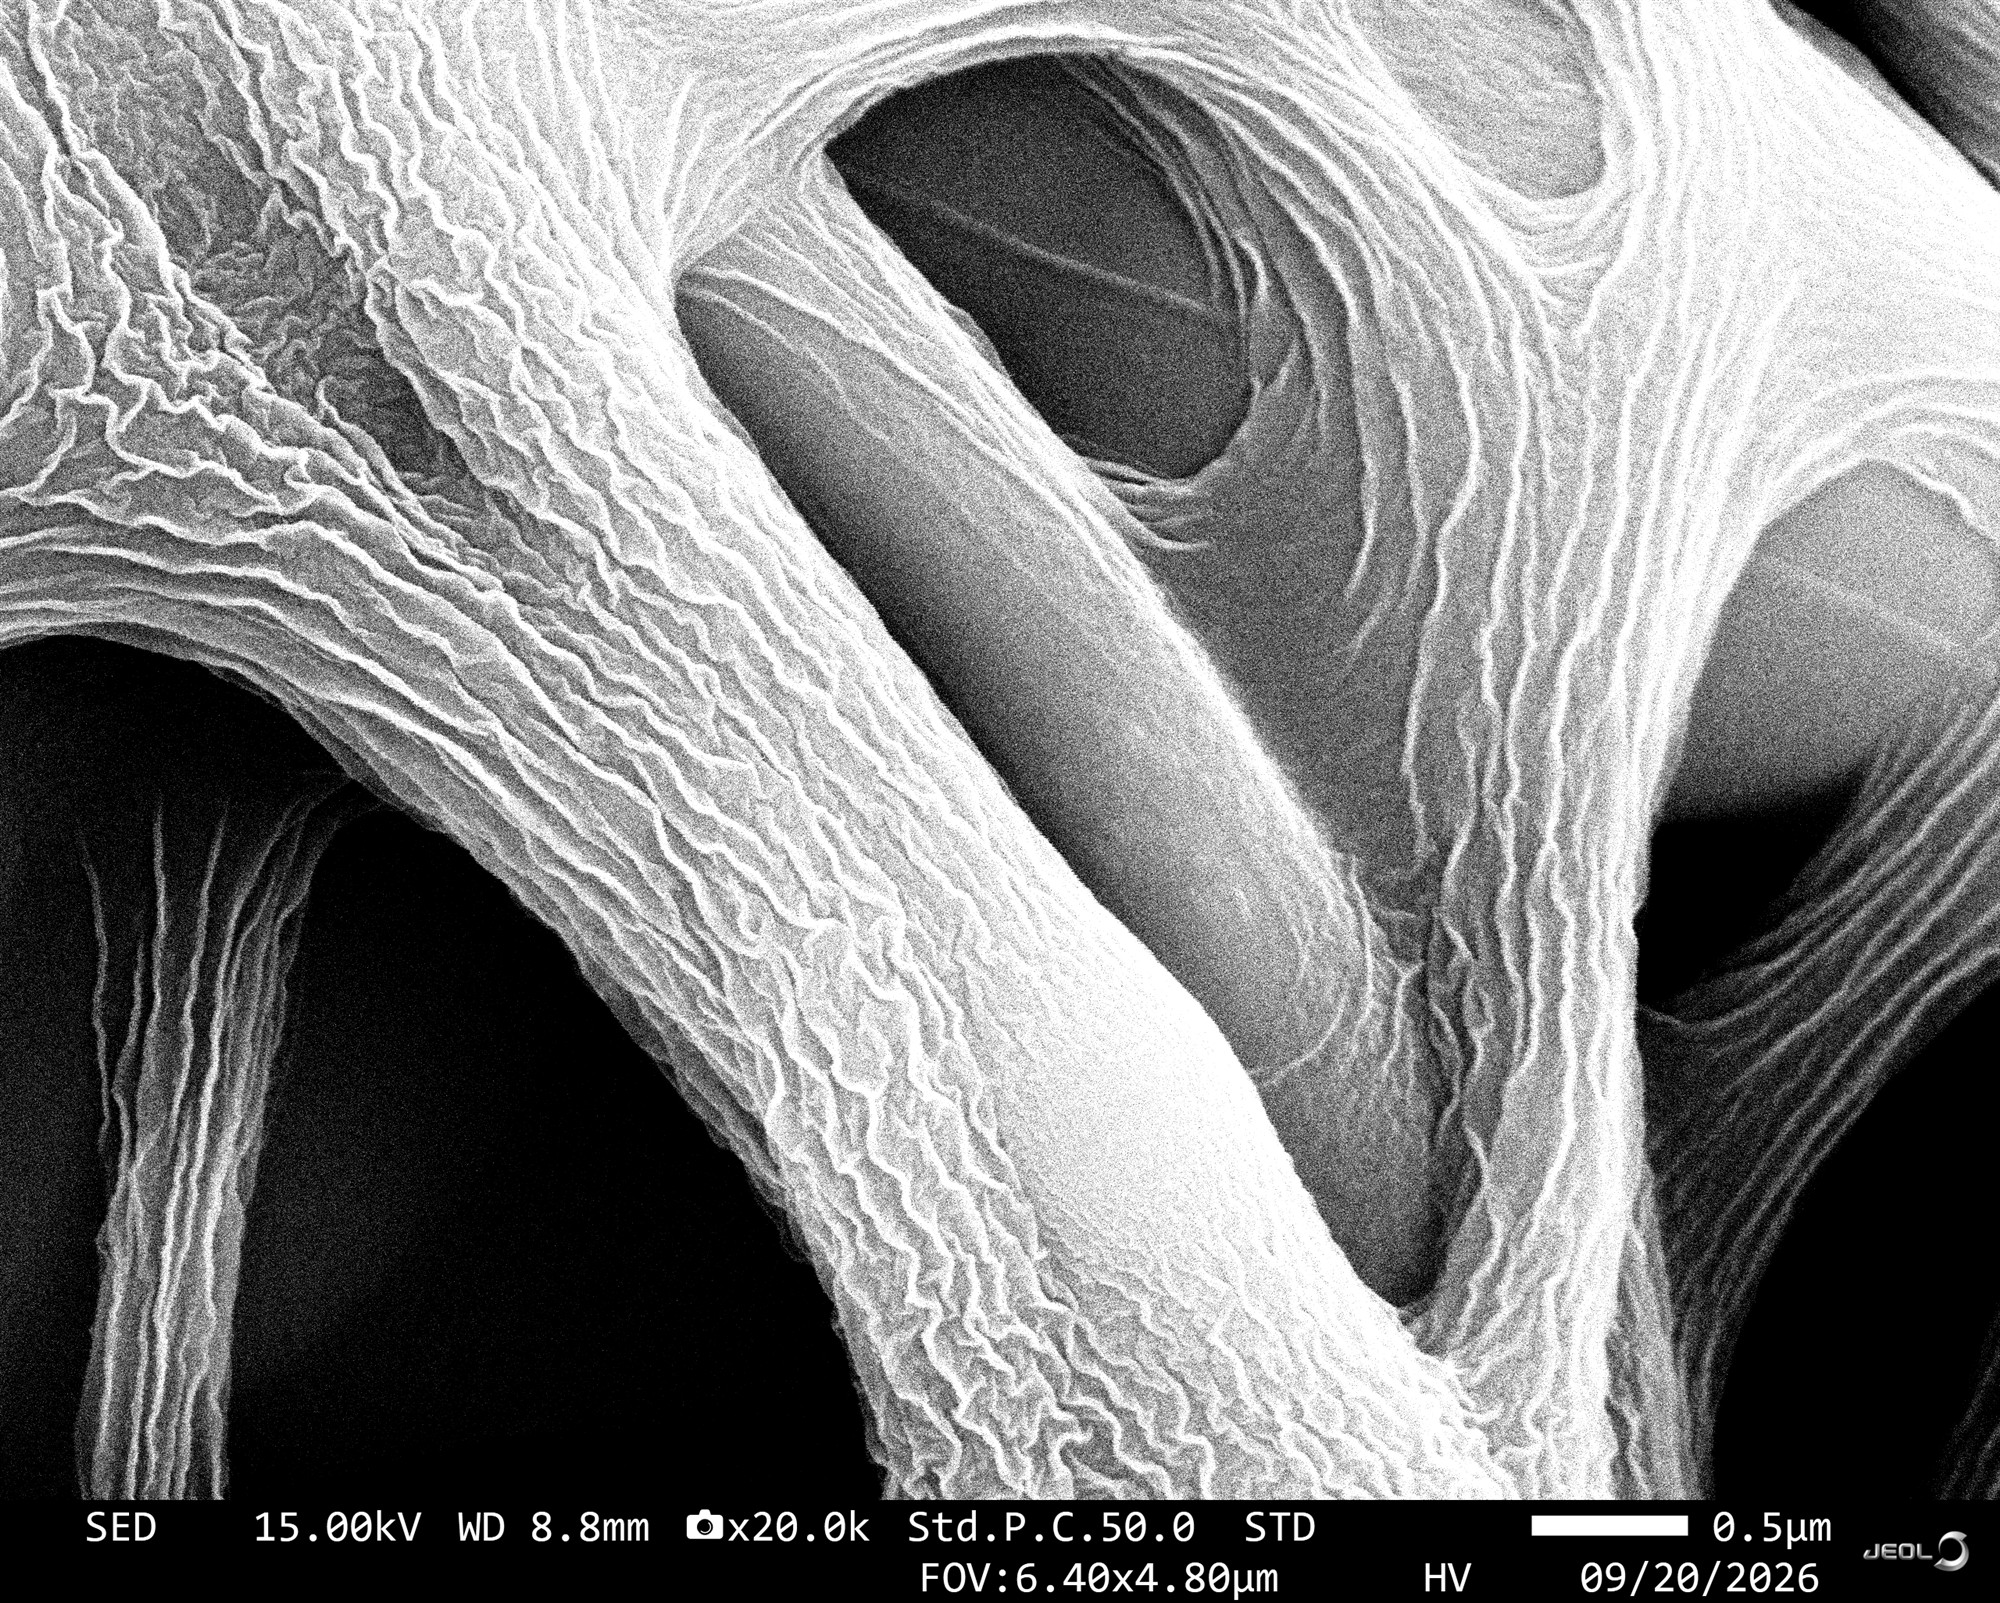
\includegraphics[width=0.48\textwidth]{picture/20260920/A_sem_20k.jpg}\hfill
    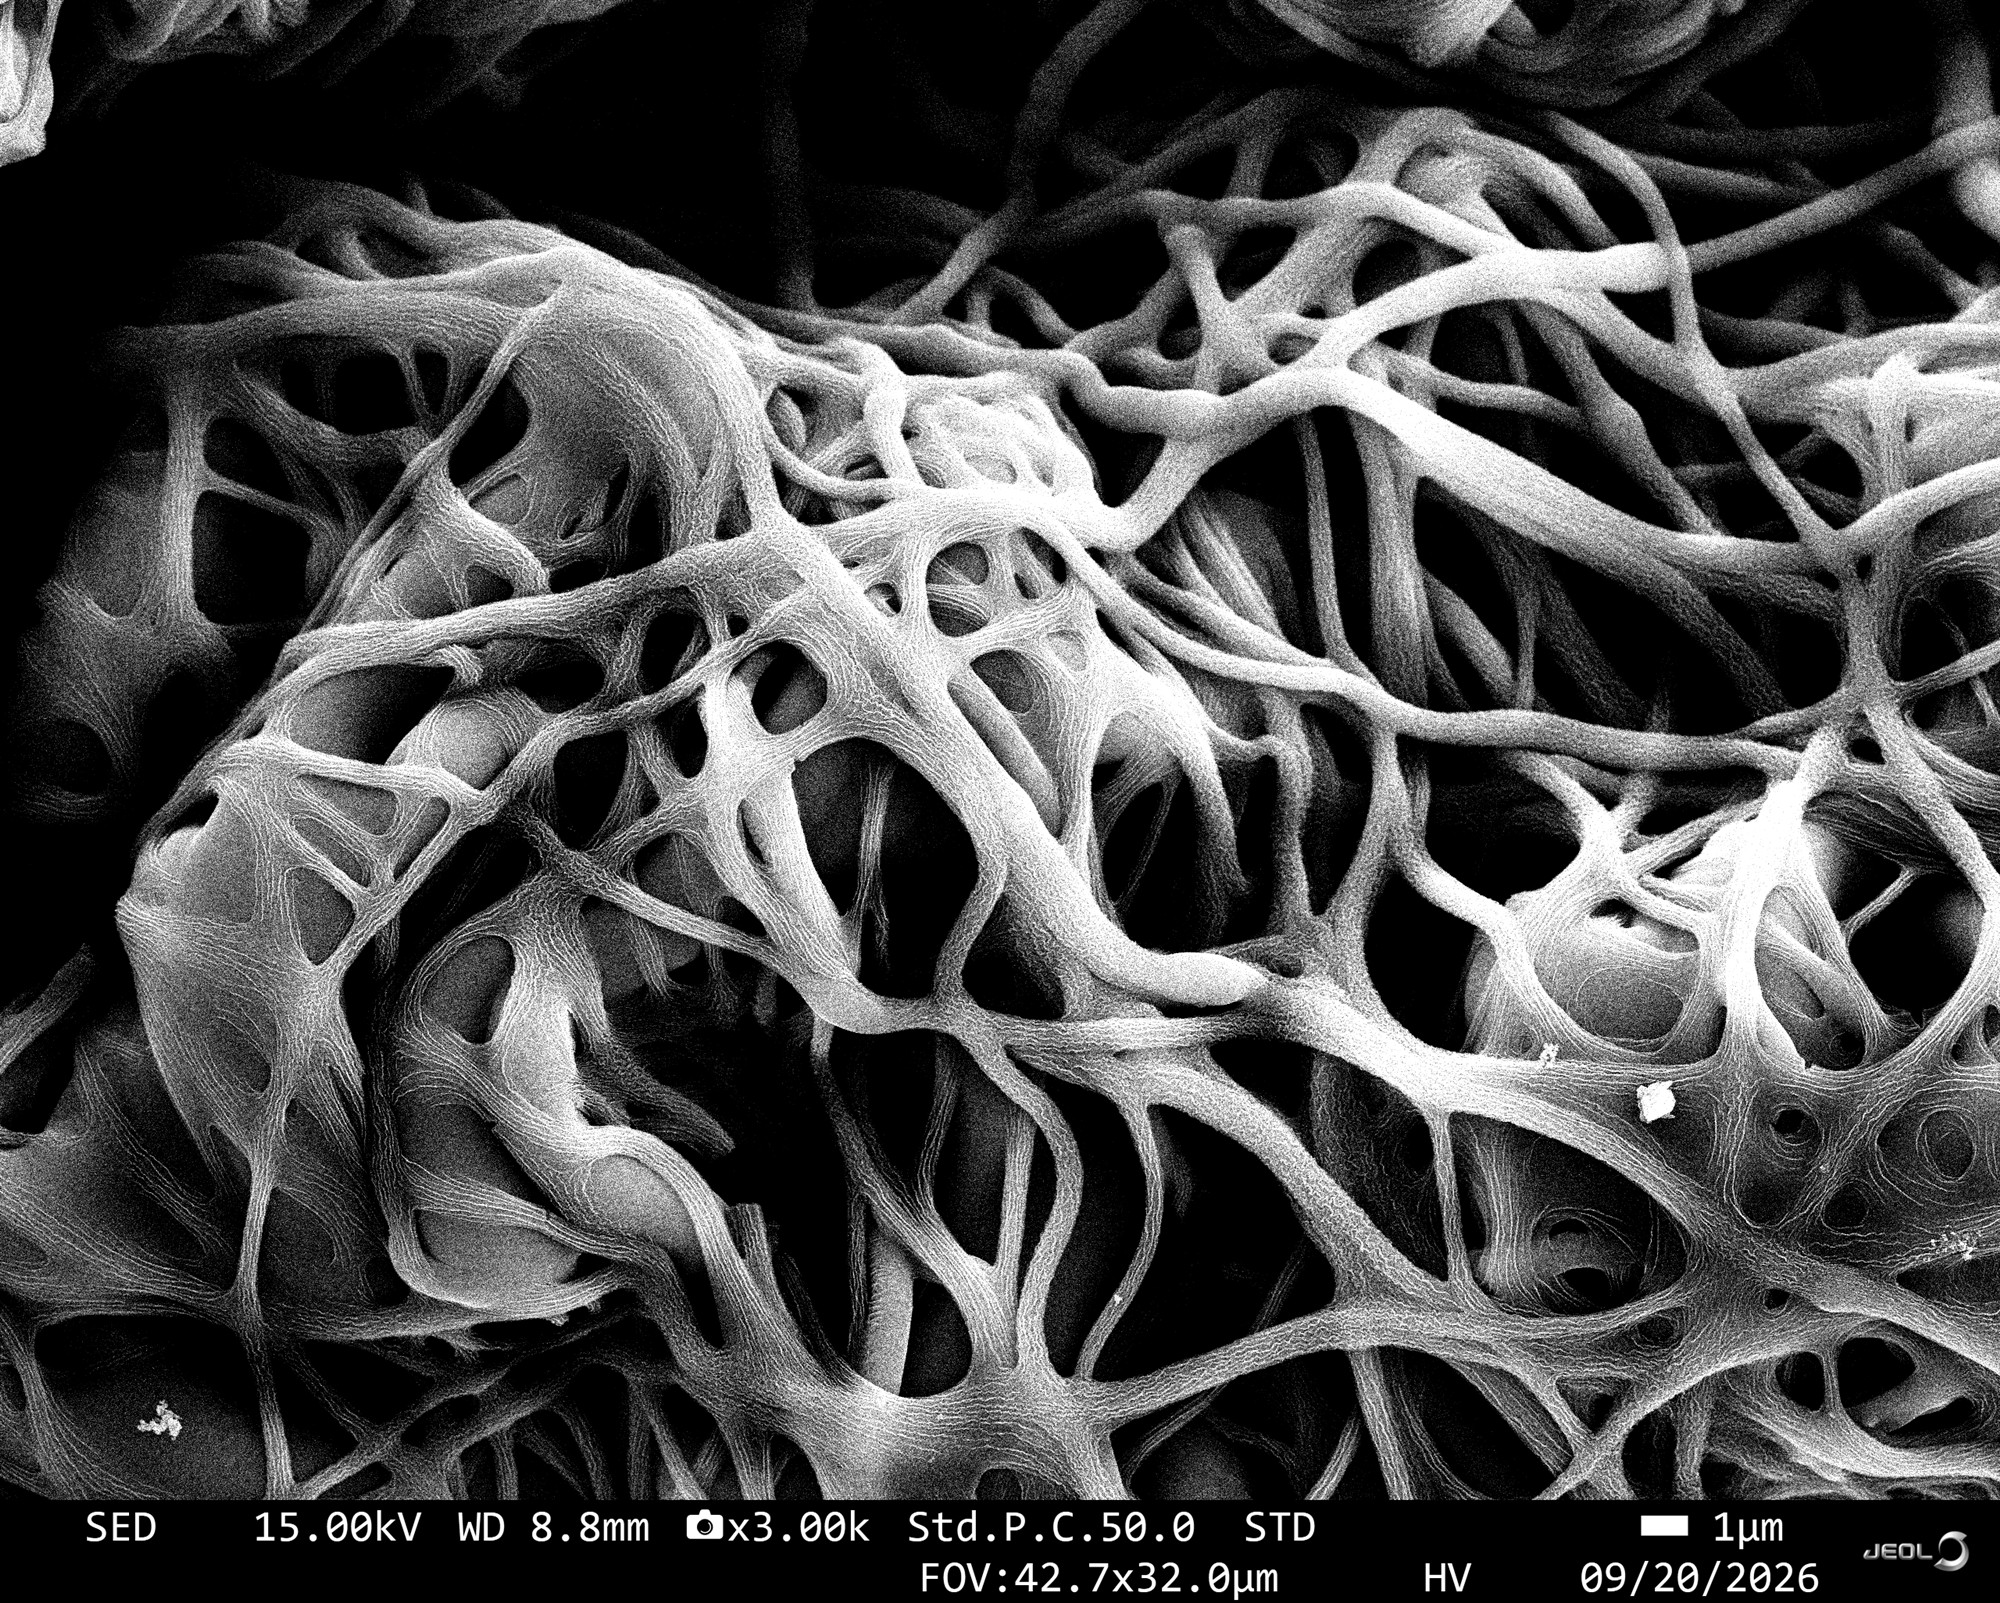
\includegraphics[width=0.48\textwidth]{picture/20260920/A_sem_3k.jpg}
    \caption{A 样（烧结后）表面形貌：左 20k（视场 6.4\,\textmu m）、右 3k（视场 42.7\,\textmu m）。连续纤维网、表面纵向沟槽，无致密膜。}
    \label{fig:A-sintered-surface}
\end{figure}

\begin{figure}[htbp]
    \centering
    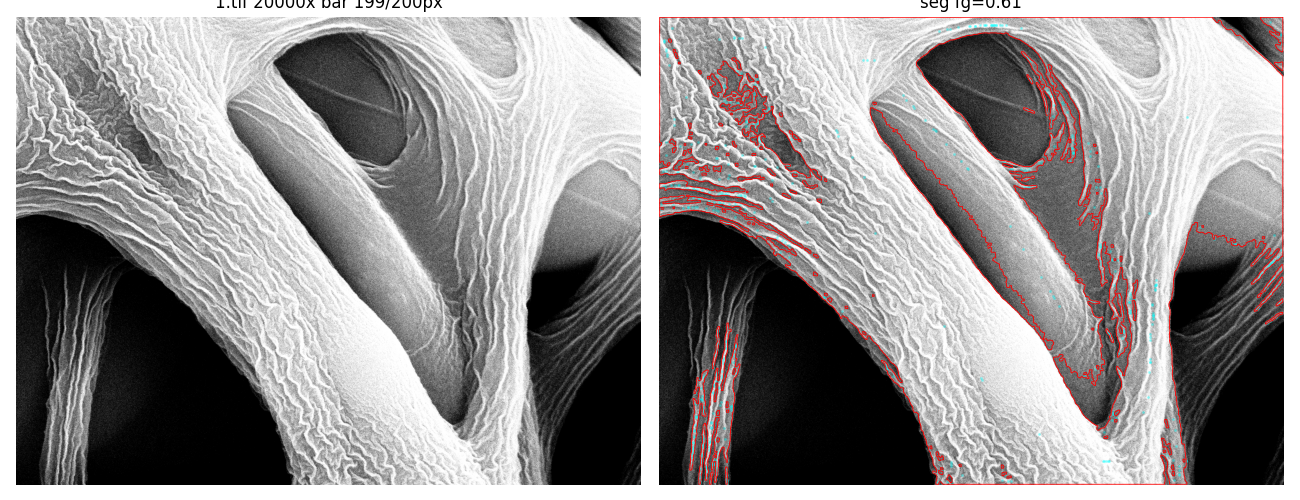
\includegraphics[width=0.48\textwidth]{picture/20260920/A_seg_20k.png}\hfill
    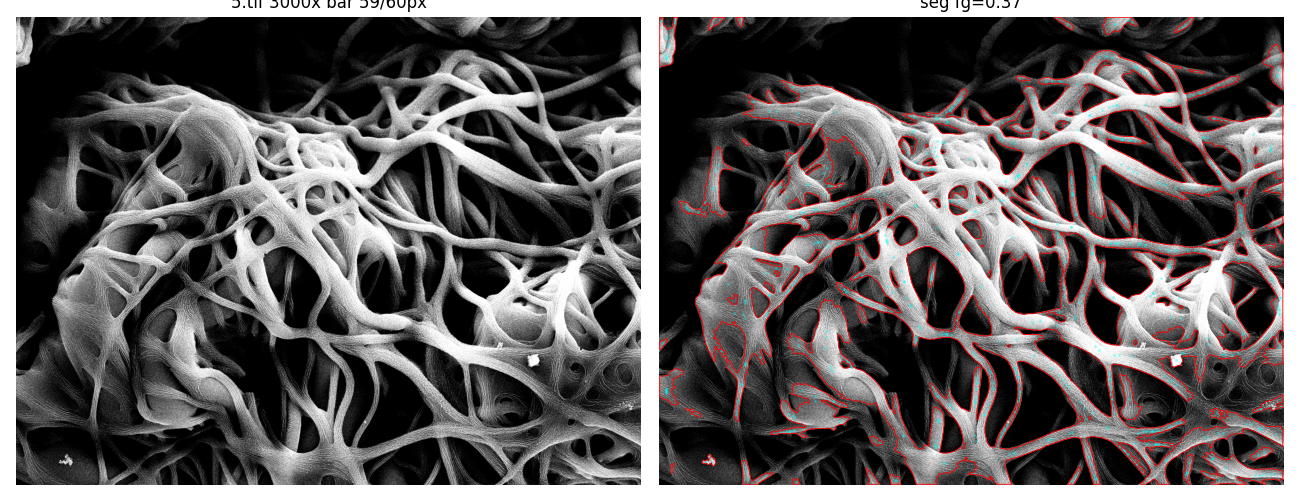
\includegraphics[width=0.48\textwidth]{picture/20260920/A_seg_3k.png}
    \caption{分割校验叠加图（左 20k，右 3k）：红色为程序识别的纤维区域，青色为距离变换脊线（纤维中心）。交汇处被连成一片会使单根直径测值偏大，故统计采用中位数。}
    \label{fig:A-seg}
\end{figure}

\begin{figure}[htbp]
    \centering
    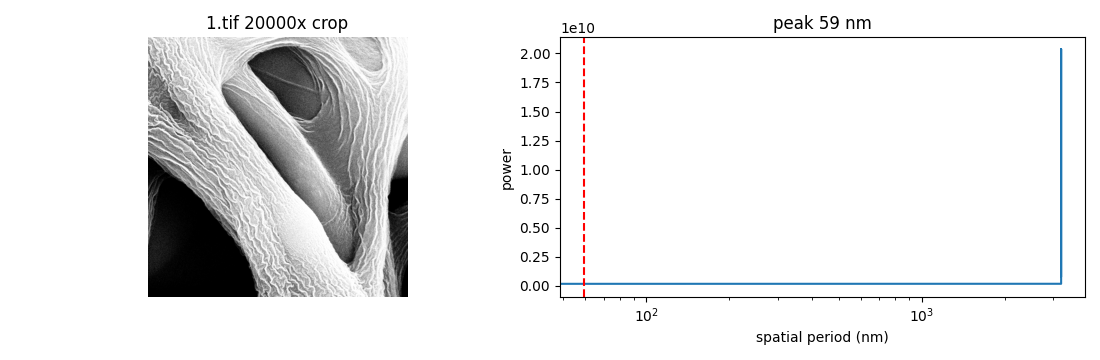
\includegraphics[width=0.48\textwidth]{picture/20260920/A_fft_20k.png}\hfill
    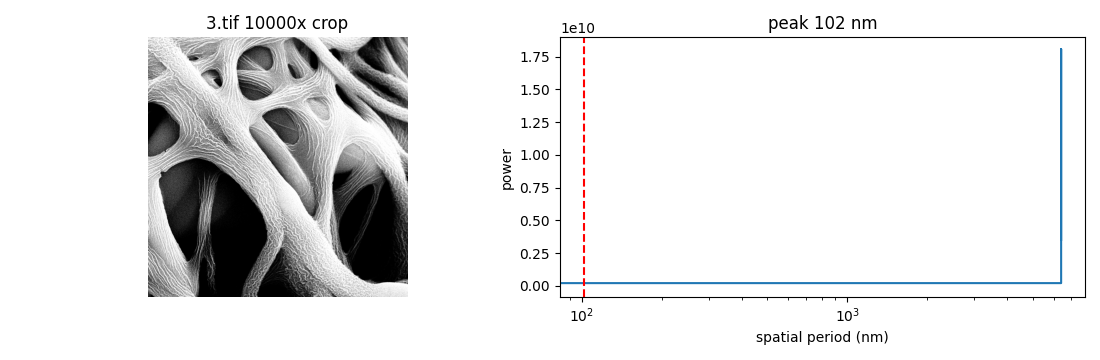
\includegraphics[width=0.48\textwidth]{picture/20260920/A_fft_10k.png}
    \caption{表面条纹间距的 FFT 径向功率谱（左 20k，右 10k），虚线标出主峰周期（45--59\,nm 与 $\approx$102\,nm）。}
    \label{fig:A-fft}
\end{figure}
